\documentclass[ignorenonframetext,]{beamer}
\usetheme{Darmstadt}
\usecolortheme{beaver}
\usefonttheme{structurebold}
\usepackage{amssymb,amsmath}
\usepackage{ifxetex,ifluatex}
\usepackage{fixltx2e} % provides \textsubscript
\usepackage{lmodern}
\ifxetex
  \usepackage{fontspec,xltxtra,xunicode}
  \defaultfontfeatures{Mapping=tex-text,Scale=MatchLowercase}
  \newcommand{\euro}{€}
\else
  \ifluatex
    \usepackage{fontspec}
    \defaultfontfeatures{Mapping=tex-text,Scale=MatchLowercase}
    \newcommand{\euro}{€}
  \else
    \usepackage[T1]{fontenc}
    \usepackage[utf8]{inputenc}
      \fi
\fi
\IfFileExists{upquote.sty}{\usepackage{upquote}}{}
% use microtype if available
\IfFileExists{microtype.sty}{\usepackage{microtype}}{}
\usepackage{letltxmacro}
\makeatletter
\def\maxwidth{\ifdim\Gin@nat@width>\linewidth\linewidth\else\Gin@nat@width\fi}
\def\maxheight{\ifdim\Gin@nat@height>\textheight0.8\textheight\else\Gin@nat@height\fi}
\makeatother
\AtBeginDocument{
  \LetLtxMacro\Oldincludegraphics\includegraphics
  \renewcommand{\includegraphics}[2][]{%
    \Oldincludegraphics[#1,width=\maxwidth,height=\maxheight,keepaspectratio]{#2}}
}

% Comment these out if you don't want a slide with just the
% part/section/subsection/subsubsection title:
\AtBeginPart{
  \let\insertpartnumber\relax
  \let\partname\relax
  \frame{\partpage}
}
\AtBeginSection{
  \let\insertsectionnumber\relax
  \let\sectionname\relax
  \frame{\sectionpage}
}
\AtBeginSubsection{
  \let\insertsubsectionnumber\relax
  \let\subsectionname\relax
  \frame{\subsectionpage}
}

\setlength{\parindent}{0pt}
\setlength{\parskip}{6pt plus 2pt minus 1pt}
\setlength{\emergencystretch}{3em}  % prevent overfull lines
\setcounter{secnumdepth}{0}

\title{Advanced Research Tools for Economics and Business Administration}
\author{Thomas de Graaff}
\date{January 8, 2015}

\begin{document}
\frame{\titlepage}

\section{Introduction}\label{introduction}

\begin{frame}{\emph{Why} this workshop?}

\begin{itemize}
\item
  In the \emph{social sciences} few attention to what tools to use (and
  why they make sense)
\item
  Increasing \emph{need} for/in openness, reproducability \&
  transparancy

  \begin{itemize}
  \itemsep1pt\parskip0pt\parsep0pt
  \item
    from journals, universities and governments
  \item
    increase in cooperation (over wider distances)
  \item
    access to your own files
  \item
    make yourself more visible
  \end{itemize}
\item
  Why \emph{I} want to give this workshop

  \begin{itemize}
  \itemsep1pt\parskip0pt\parsep0pt
  \item
    intrinsic interest
  \item
    my goal: pre-conferences workshops / courses
  \end{itemize}
\end{itemize}

\end{frame}

\begin{frame}{What I want (and don't want) with this workshop}

\begin{itemize}
\item
  Give a general introduction of why some tools work together

  \begin{itemize}
  \itemsep1pt\parskip0pt\parsep0pt
  \item
    Why version control systems?
  \item
    Why reference managers
  \end{itemize}
\item
  Give an introduction to \LaTeX

  \begin{itemize}
  \itemsep1pt\parskip0pt\parsep0pt
  \item
    First the basics
  \item
    Next workshop: some advanced stuff
  \end{itemize}
\item
  What \emph{I} do not want

  \begin{itemize}
  \itemsep1pt\parskip0pt\parsep0pt
  \item
    Tell you what applications to use (\textbf{you} need to decide and
    make a \textbf{well-informed} decision)
  \end{itemize}
\end{itemize}

\end{frame}

\section{Workflow}\label{workflow}

\begin{frame}{Research cycle}

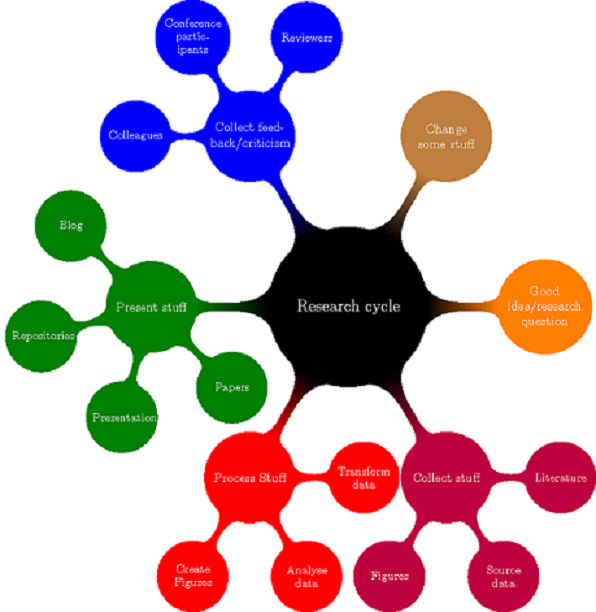
\includegraphics{fig/ResearchCycle.png}

\end{frame}

\begin{frame}{Why bother about a workflow or tools?}

\begin{itemize}
\item
  Good scientific practice: \emph{document how you have achieved your
  results}; this ensures

  \begin{itemize}
  \itemsep1pt\parskip0pt\parsep0pt
  \item
    Reproducibility
  \item
    Transparency
  \item
    Modularity
  \item
    Portability (across systems and users)
  \item
    Efficiency
  \item
    Self-sanity
  \end{itemize}
\end{itemize}

\end{frame}

\begin{frame}{When should I adopt new tools/workflow?}

\begin{itemize}
\itemsep1pt\parskip0pt\parsep0pt
\item
  The sooner the better (you really have time now)
\item
  But think twice about which one (switching is costly; not in terms of
  beer but in terms of time)
\item
  Start one step at a time (starting with \LaTeX is a pretty neat idea)
\end{itemize}

\emph{A journey of a thousand miles begins with a single step}

Lao-tzu

\end{frame}

\begin{frame}{In general}

\begin{quote}
In science consensus is irrelevant. What is relevant is reproducible
results. The greatest scientists in history are great precisely because
they broke with the consensus (Michael Crichton)
\end{quote}

\end{frame}

\begin{frame}{In data science}

\begin{itemize}
\item
  Typically, a publication is not at the heart of research

  \begin{itemize}
  \itemsep1pt\parskip0pt\parsep0pt
  \item
    Code
  \item
    Data
  \end{itemize}
\end{itemize}

\begin{quote}
The data and code used to make a finding are available and they are
sufficient for an independent researcher to recreate the finding (Peng,
2011)
\end{quote}

\end{frame}

\begin{frame}{Code, documentation and output}

\begin{enumerate}
\def\labelenumi{\arabic{enumi}.}
\item
  Synonyms
\item
  All based on \texttt{.txt} files
\item
  Encompasses almost anything

  \begin{itemize}
  \itemsep1pt\parskip0pt\parsep0pt
  \item
    data itself (\texttt{.csv})
  \item
    set of commands for data cleaning and statistical analysis
    (\texttt{.do}, \texttt{.R})
  \item
    database with references (\texttt{.bib})
  \item
    transcript of interviews (\texttt{.tex})
  \item
    text for aticles, presentations or websites (\texttt{.tex},
    \texttt{.html})
  \end{itemize}
\item
  Only output is displayed/interpreted differently (e.g., in a browser
  or pdf viewer)
\end{enumerate}

\end{frame}

\begin{frame}{Tools for workflows in this workshop}

\begin{itemize}
\item
  Versioning system (Time-Machine, Dropbox, GitHub)
\item
  Reference manager (Mendeley)
\item
  Markup lanaguages

  \begin{itemize}
  \itemsep1pt\parskip0pt\parsep0pt
  \item
    \LaTeX 
  \item
    HTML
  \end{itemize}
\end{itemize}

\end{frame}

\section{Version Control Systems}\label{version-control-systems}

\begin{frame}{Folder structure of your new project (theses, paper,
research)}

\begin{itemize}
\item
  Think \emph{a priori} about project set-up

  \begin{itemize}
  \itemsep1pt\parskip0pt\parsep0pt
  \item
    Seperate analysis, data and output files
  \end{itemize}
\item
  Be careful with source data!

  \begin{itemize}
  \item
    Seperate source and derived data files
  \item
    Typically

    \begin{itemize}
    \itemsep1pt\parskip0pt\parsep0pt
    \item
      you get/collect data
    \item
      transform data
    \item
      analyse data
    \end{itemize}
  \item
    Keep track of all these stages!
  \end{itemize}
\end{itemize}

\end{frame}

\begin{frame}{Why is version control systems such a neat idea}


\includegraphics{fig/phdcomic.png}

\end{frame}

\begin{frame}{Version control systems}

With version control system only one copy of each file (but with fully
backed-up history)

A version control system is not the same as a backup devise, but the
combination is a killer-ap

\begin{itemize}
\item
  Time machine (mac only) with external hard drive
\item
  Dropbox
\item
  more advanced stuff: Git and GitHub
\end{itemize}

With \texttt{.txt} files you can use the \texttt{diff} command

\end{frame}

\section{Reference managers}\label{reference-managers}

\begin{frame}{Why reference managers?}

This is a life saver!

\begin{quote}
Use one!
\end{quote}

Several applications out there:

\begin{itemize}
\itemsep1pt\parskip0pt\parsep0pt
\item
  In this case Mendeley (free but not open source)
\item
  Make sure it exports to \texttt{.bib} files
\item
  Search for references (google scholar, jstor, etc.)
\item
  Mendeley can import \texttt{.pdf}'s
\end{itemize}

\end{frame}

\section{\LaTeX}\label{section}

\begin{frame}{Background}

\begin{itemize}
\item
  \TeX has been devised by Donald E. Knuth in the late 70's
\item
  \LaTeX is a set of macro's around TeX and devised in the 80's
\item
  \LaTeX is a \emph{typesetting program}, not a \emph{Word processor}

  \begin{itemize}
  \itemsep1pt\parskip0pt\parsep0pt
  \item
    It is actually some code that needs to be compiled
  \item
    Code is typed in by an editor
  \end{itemize}
\item
  So, huge differences between

  \begin{itemize}
  \item
    Word processor: Open Office, Word
  \item
    Typesetter: \LaTeX, Adobe's InDesign (in general XML)
  \item
    Editors:

    \begin{itemize}
    \itemsep1pt\parskip0pt\parsep0pt
    \item
      Specific editors: TexStudio, TexShop, RStudio
    \item
      General editors: Sublime, TextMate, Notepad++, Vim, Emacs
    \end{itemize}
  \end{itemize}
\end{itemize}

\end{frame}

\begin{frame}{Disadvantages}

\begin{itemize}
\item
  Not WYSIWYG
\item
  You nead to learn (quite) some commands

  \begin{itemize}
  \itemsep1pt\parskip0pt\parsep0pt
  \item
    Learning curve, but
  \item
    hurray for
    \href{http://www.stdout.org/~winston/latex/latexsheet-a4.pdf}{cheat
    sheets} and Google
  \end{itemize}
\item
  Very specific lay-outs difficult to attain
\item
  Basic \LaTeX has \emph{difficulties} with incorporating new fonts
  (Hoefler, minion pro)

  \begin{itemize}
  \itemsep1pt\parskip0pt\parsep0pt
  \item
    XeTeX
  \item
    For the purists: \LaTeX does it right
    \href{http://oestrem.com/thingstwice/2007/05/latex-vs-word-vs-writer/}{(\LaTeX vs
    Word)}
  \end{itemize}
\end{itemize}

\end{frame}

\begin{frame}{Advantages}

\begin{itemize}
\itemsep1pt\parskip0pt\parsep0pt
\item
  Free (as in beer) and ubiquitous
\item
  WYSIWYM
\item
  Consistent lay-out throughout the whole document (including tables,
  appendices, formulas, source code, etc)
\item
  Internal references are a breeze (references, tables of, indices)
\item
  Forced to structure documents
\item
  Macros, thus scriptable
\item
  Large community, thus a package for almost everything (books,
  articles, presentation, posters, exams, musicscores)
\item
  Superior typography \& output
\item
  Large publishers (i.e., Elsevier and Springer) have \LaTeX templates
  for their articles
\end{itemize}

\end{frame}

\begin{frame}{How does it work in practice?}

\begin{itemize}
\item
  You edit a \texttt{.tex} file without thinking about how it looks

  \begin{itemize}
  \itemsep1pt\parskip0pt\parsep0pt
  \item
    distraction free writing (yeah right)
  \end{itemize}
\item
  You then compile it

  \begin{itemize}
  \itemsep1pt\parskip0pt\parsep0pt
  \item
    \LaTeX is unforgiving: if there is an error, usually it does not
    compile
  \item
    Typically, errors are missing brackets or parentheses.
  \end{itemize}
\item
  Typically, source \texttt{.tex} file is compiled into \texttt{.pdf}
\end{itemize}

\end{frame}

\begin{frame}[fragile]{Basic set-up}

\begin{verbatim}
\documentclass[]{article}
%opening
\title{}
\author{}

\begin{document}

\maketitle

\begin{abstract}
\end{abstract}

\section{}

\end{document}
\end{verbatim}

\end{frame}

\begin{frame}{Creating some text}

\begin{itemize}
\item
  Use a first package: \texttt{\textbackslash{}usepackage\{lipsum\}}
\item
  Create an abstract, title, authors and will in some sections
\item
  Create subsections
\end{itemize}

\end{frame}

\begin{frame}{Further text control}

\begin{itemize}
\item
  itemization
\item
  enumeration
\item
  bold
\item
  emphasize
\end{itemize}

\end{frame}

\begin{frame}[fragile]{Inserting equations}

\begin{itemize}
\itemsep1pt\parskip0pt\parsep0pt
\item
  Inline: \$e=mc\^{}2\$ will be $e=mc^2$
\end{itemize}

or

\begin{verbatim}
\begin{equation}
e=mc^2
\end{equation}
\end{verbatim}

will render in

\[
e=mc^2
\]

\begin{itemize}
\itemsep1pt\parskip0pt\parsep0pt
\item
  Equations can be as complex (cool) as you want
\end{itemize}

\end{frame}

\begin{frame}[fragile]{Inserting figures}

\begin{verbatim}
\usepackage{graphicx}

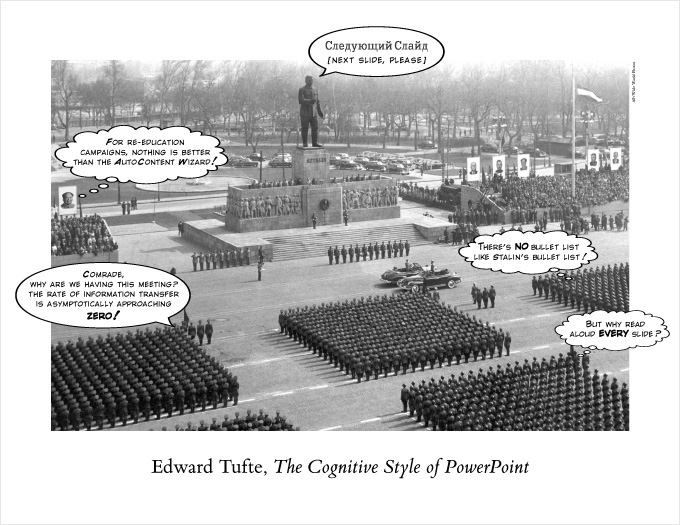
\includegraphics{../Figs/home_stalin_poster}
\end{verbatim}

Better is to include them in a floating environment (this is where
typically the problem starts)

\begin{verbatim}
\begin{figure}[htb!]
    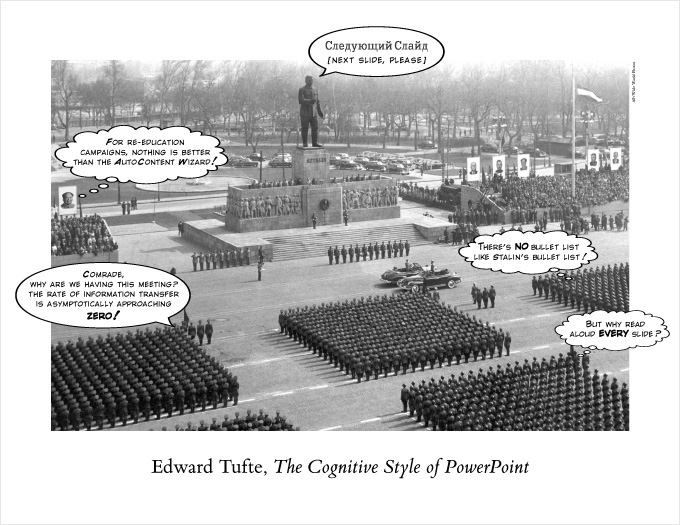
\includegraphics[width = 1.0\textwidth]
    {../Figs/home_stalin_poster}
    \caption{Next slide please!}
\end{figure}
\end{verbatim}

\end{frame}

\begin{frame}[fragile]{Inserting tables}

\begin{itemize}
\itemsep1pt\parskip0pt\parsep0pt
\item
  Within a table environment and most basic with tabubar, so:
\end{itemize}

\begin{verbatim}
\begin{table}[h!]
    \caption{Who is afraid of ...}
    \label{tab:colors}
    \begin{tabular}{ccc} 
        \hline
            1   & 2      & 3 \\ 
        \hline
            red & yellow & blue 
        \hline
    \begin{tabular}
\end{table}
\end{verbatim}

\end{frame}

\end{document}
